\subsection{Excercise UMEGeneralConcepts}
\label{sec:ume_general_concepts}
%//TODO: Kurze Einleitung
\subsubsection*{Architectural Style}
The Unified Microservice Engineering approach aligns with the microservices architectural style.
This involves breaking down an application into smaller, independent services that can be developed, deployed, and scaled separately.
The services communicate with each other through APIs and are usually organized around business capabilities.
These services aim to enhance flexibility, scalability, and maintainability.

Predecessors of the microservices architectural style are the service-oriented architecture (SOA) and the distributed systems architectural style which will be further explained in the following.

\paragraph*{Service Oriented Architecture}
SOA shares some similarities with the microservices architectural style.
The focus is on organizing services around business capabilities and developing them independently.
This aims to achieve reusability and interoperability.

Yet, microservices tend to be generally smaller, more fine-grained, decoupled and are usually lightweight.

\paragraph*{Distributed Systems}
Distributed systems represent a collection of independent computers, appearing to the users of the system as a single coherent system.
These systems handle tasks across a network, each node having its local memory and set of responsibilities.

Microservices share a similar idea: Splitting an application into smaller, more independent services communicating with each other.
Each microservice manages its functionalities and data to provide the overall functionality of the application.

\subsubsection*{Domain Modelling}
A domain model describes selected aspects of a domain in a conceptual model, yet the model should not separate the concept from the implementation.
This model can be used to better understand the domain and to communicate with stakeholders.

The domain model is located in the domain logic layer of the layered architecture.
Therefore each microservice implements its domain model.

Using a layered software architecture, the business logic layer is separated into application logic and domain logic.
The application logic layer contains the application-specific logic while the domain logic layer contains the domain-specific logic.
This domain-specific logic is derived from the domain model, enabling the domain knowledge to be encapsulated in the domain logic layer.
The application logic layer is derived from the analysis of the application requirements, for instance, use cases.

Therefore the domain logic layer is the part of the software architecture that is shaped the most by domain modeling.

\subsubsection*{Modelling of the Architecture}
To model the architecture of a microservice-based application, UME uses the Unified Modeling Language (UML).
To create the according diagrams, the UMLet tool is used.

Two modeling views can be distinguished: the tactical and the strategic view.

The strategic modeling provides an overview of the domain model.
The result is the so-called context map.
It provides the link to the microservice architecture.
The context map consists of subdomains and their bounded contexts.
A bounded context can be seen as a microservice candidate.

Tactical modeling takes a closer look at the entities and their relationships.
Each bounded context entity models the static relations of the domain entity.

\subsection{Excercise APIStyles}
\label{sec:api_styles}
%//TODO: Kurze Einleitung
\subsubsection*{REST and gRPC}
Representational state Transfer (REST) and Remote Procedure Call (gRPC) are two different frameworks and collections of best practices and technologies for building APIs.

The main conceptual difference is the focus and orientation of both concepts:
REST is resource-oriented.
Each resource has a unique identifier (URI) and can be accessed using the standardized HTTP methods.
Therefore, there is only a small set of well-defined methods for manipulating the resources.
gRPC is procedure, method, or function-oriented.
It is based on the idea of implementing a service, offering remotely callable methods.
These methods can be called by a client with their parameters and return values.

Both concepts have their legitimate use cases, yet it is important to choose the right one for the given use case.

\subsubsection*{REST Properties}
REST provides a concept of how microservices' APIs should be designed.
Its main properties are explained in the following.

\paragraph*{Addressable Ressources:}
As mentioned before, REST is resource-oriented meaning that each resource has a unique identifier, a URL, and can be accessed using the standardized HTTP methods.
Therefore only a small set of functions is needed to manipulate the resources, offering a uniform interface.

\paragraph*{Stateless Communication:}
REST is stateless meaning that each request is independent of the previous one.
The server, therefore, does not need to store any information about the client.
The client must transfer all the information in the request that is needed to process it to the server.
This leads to a loss of performance.
Yet, this is a tradeoff for an increase in scalability and robustness.

\paragraph*{Representation Orientation:}
This principle strongly relates to resources.
These resources have to be represented.
This happens in a standardized format, for instance, JSON or XML.
The client can choose the format that suits him best.
MIME, the Multipurpose Internet Mail Extensions standard, defines the different formats used in internet protocols.

\subsubsection*{gRPC Components}
% Name and describe the main components of the gRPC architecture.
gRPC is an open-source remote procedure call system, a competitive alternative to REST.
As mentioned above, gRPC is based on the idea of defining a service and specifying remotely callable methods.

\autoref{fig:grpc_main_components} shows the main components that will be explained in the following.
\paragraph*{Proto File:}
The proto file defines the service and the methods that can be called remotely.
Before calling a method, a stub needs to be generated.
This stub is generated from the proto file and contains the method signatures.

\paragraph*{Client:}
The client is the caller of the remote methods.
It uses the stub to call the methods.
The communication between the client and the server uses protobuf messages via HTTP/2.

\paragraph*{Server:}
The server is the receiver of the remote method calls.
It implements the methods defined in the proto file.
After receiving a call, the server executes the method and returns the result to the client.

\begin{figure}
    \centering
    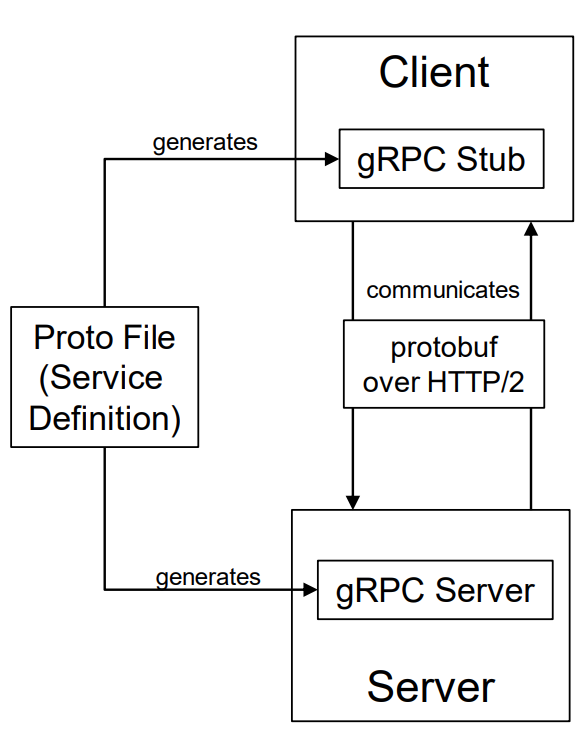
\includegraphics[width=0.4\textwidth]{figures/microservices/microservices_grpcMainComponents.png}
    \caption{Main Components of the gRPC Architecture}
    \label{fig:grpc_main_components}
\end{figure}

\subsubsection*{Use of REST and gRPC in UME}
% //TODO: Which API style is appropriate for which type of microservice in the UME approach?

\subsection{Excercise ArchitectureCarRentalAppV1.0}
\label{sec:architecture_car_rental_app_v1_0}
%//TODO: Kurze Einleitung